% **************************************************************************** %
%                                                                              %
%                                                     ::::::::  :::::::::      %
%    sec_intro.tex                                      :+:      :+:    :+:    %
%                                                    +:+        +:+    +:+     %
%    By: A. Campo <andoitzcp@gmail.com>              +#+        +#++:++#+      %
%                                                    +#+        +#+            %
%    Created: 2022/11/18 22:55:54 by A. Campo        #+#    #+# #+#            %
%    Updated: 2023/02/16 04:35:39 by acampo-p         ###   ########.fr        %
%                                                                              %
% **************************************************************************** %

\section{INTRODUCCIÓN}\label{sec:intro}

El sector de la automoción,
engloba una gran variedad de industria y servicios dedicados a servirla.
Se estima que la aportación económica total de las actividades relacionadas,
en este sector, asciende a un 11\% del PIB,
lo que la convierte en la industria manufacturera que más ingresos aporta
después  del 18,8\% del PIB que posee la industria agroalimentaria española
\citep{caixabank2021analisis}.

En este sector, el vehículo de propulsión autónoma,
es generalmente utilizado tanto por los servicios de transporte a pasajero,
como por los servicios logísticos dedicados al transporte de mercancías.
Entre los componentes que forman el vehículo autónomo,
se encuentran las cubiertas o neumáticos,
los cuales se comportan como enlace entre el vehículo y el pavimento.
Este nexo permite una transmisión eficiente
de la energía producida por el motor de combustión interna,
y a su vez, sus propiedades elásticas atenúan las irregularidades de la vía.

La industria manufacturera de cubiertas,
ha mantenido un incremento sostenido en su producción en los últimos años,
como puede observarse en la Figura \ref{fig:1_global_prod_evo}.
El mercado de neumáticos es liderado por dos empresas: Bridgestone y Michelin
\citep{rodgers2020tire}.
Las demás empresas compiten entre ellas
a una magnitud inferior a los líderes del sector,
como se aprecia en la Figura \ref{fig:1_brand_revenue}.

\begin{figure}[h]
	\begin{center}
		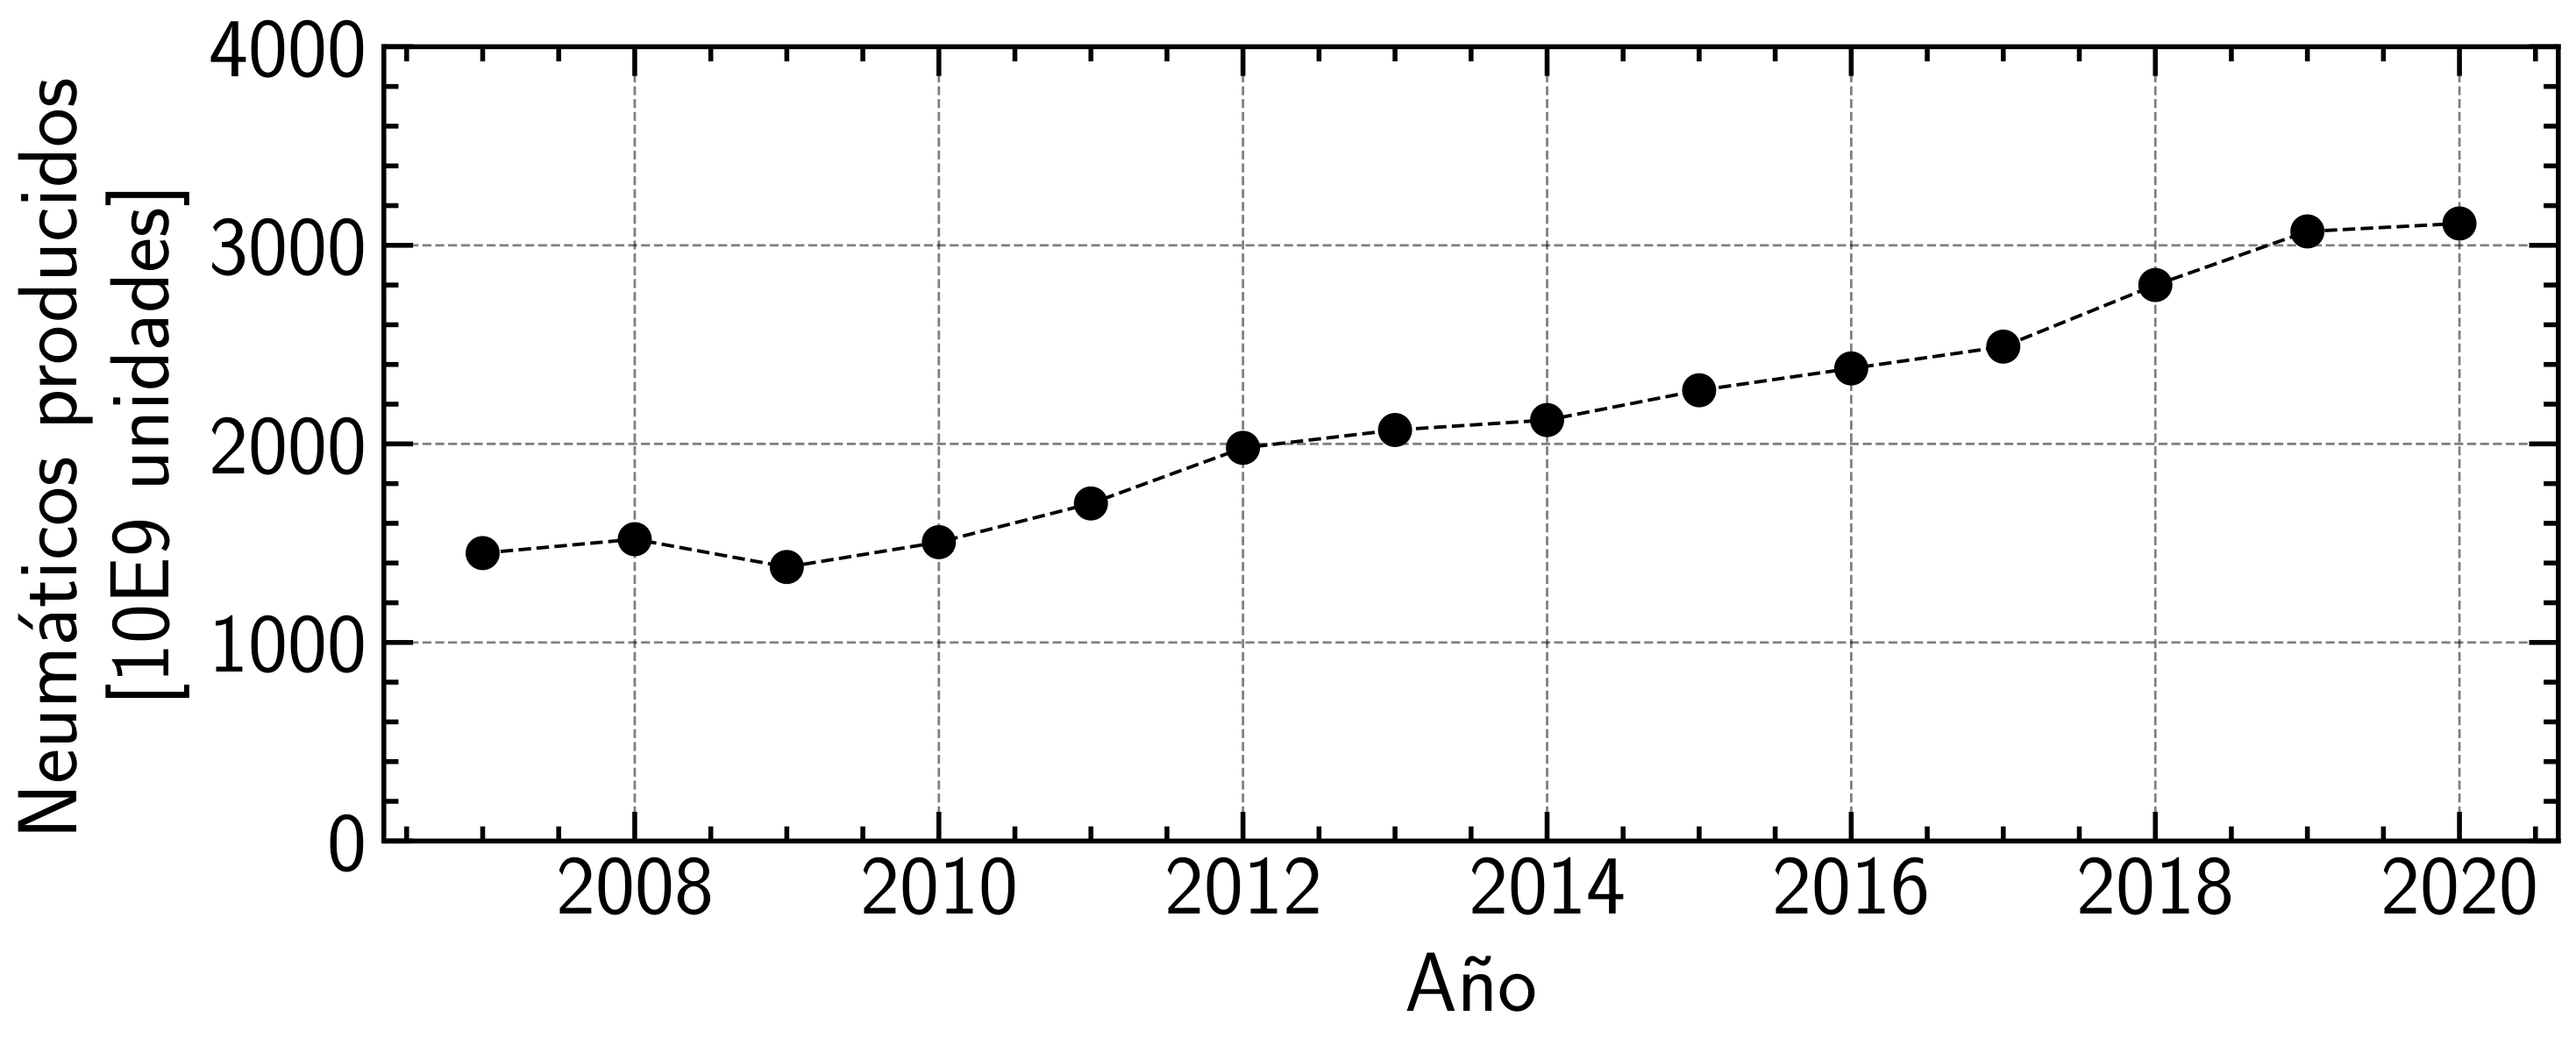
\includegraphics[width=\textwidth]{fig/1_global_prod_evo.PNG}
	\end{center}
	\caption{Evolución de la producción mundial de cubiertas \citep{rodgers2020tire}.}
	\label{fig:1_global_prod_evo}
\end{figure}

 \begin{figure}[h]
	\begin{center}
		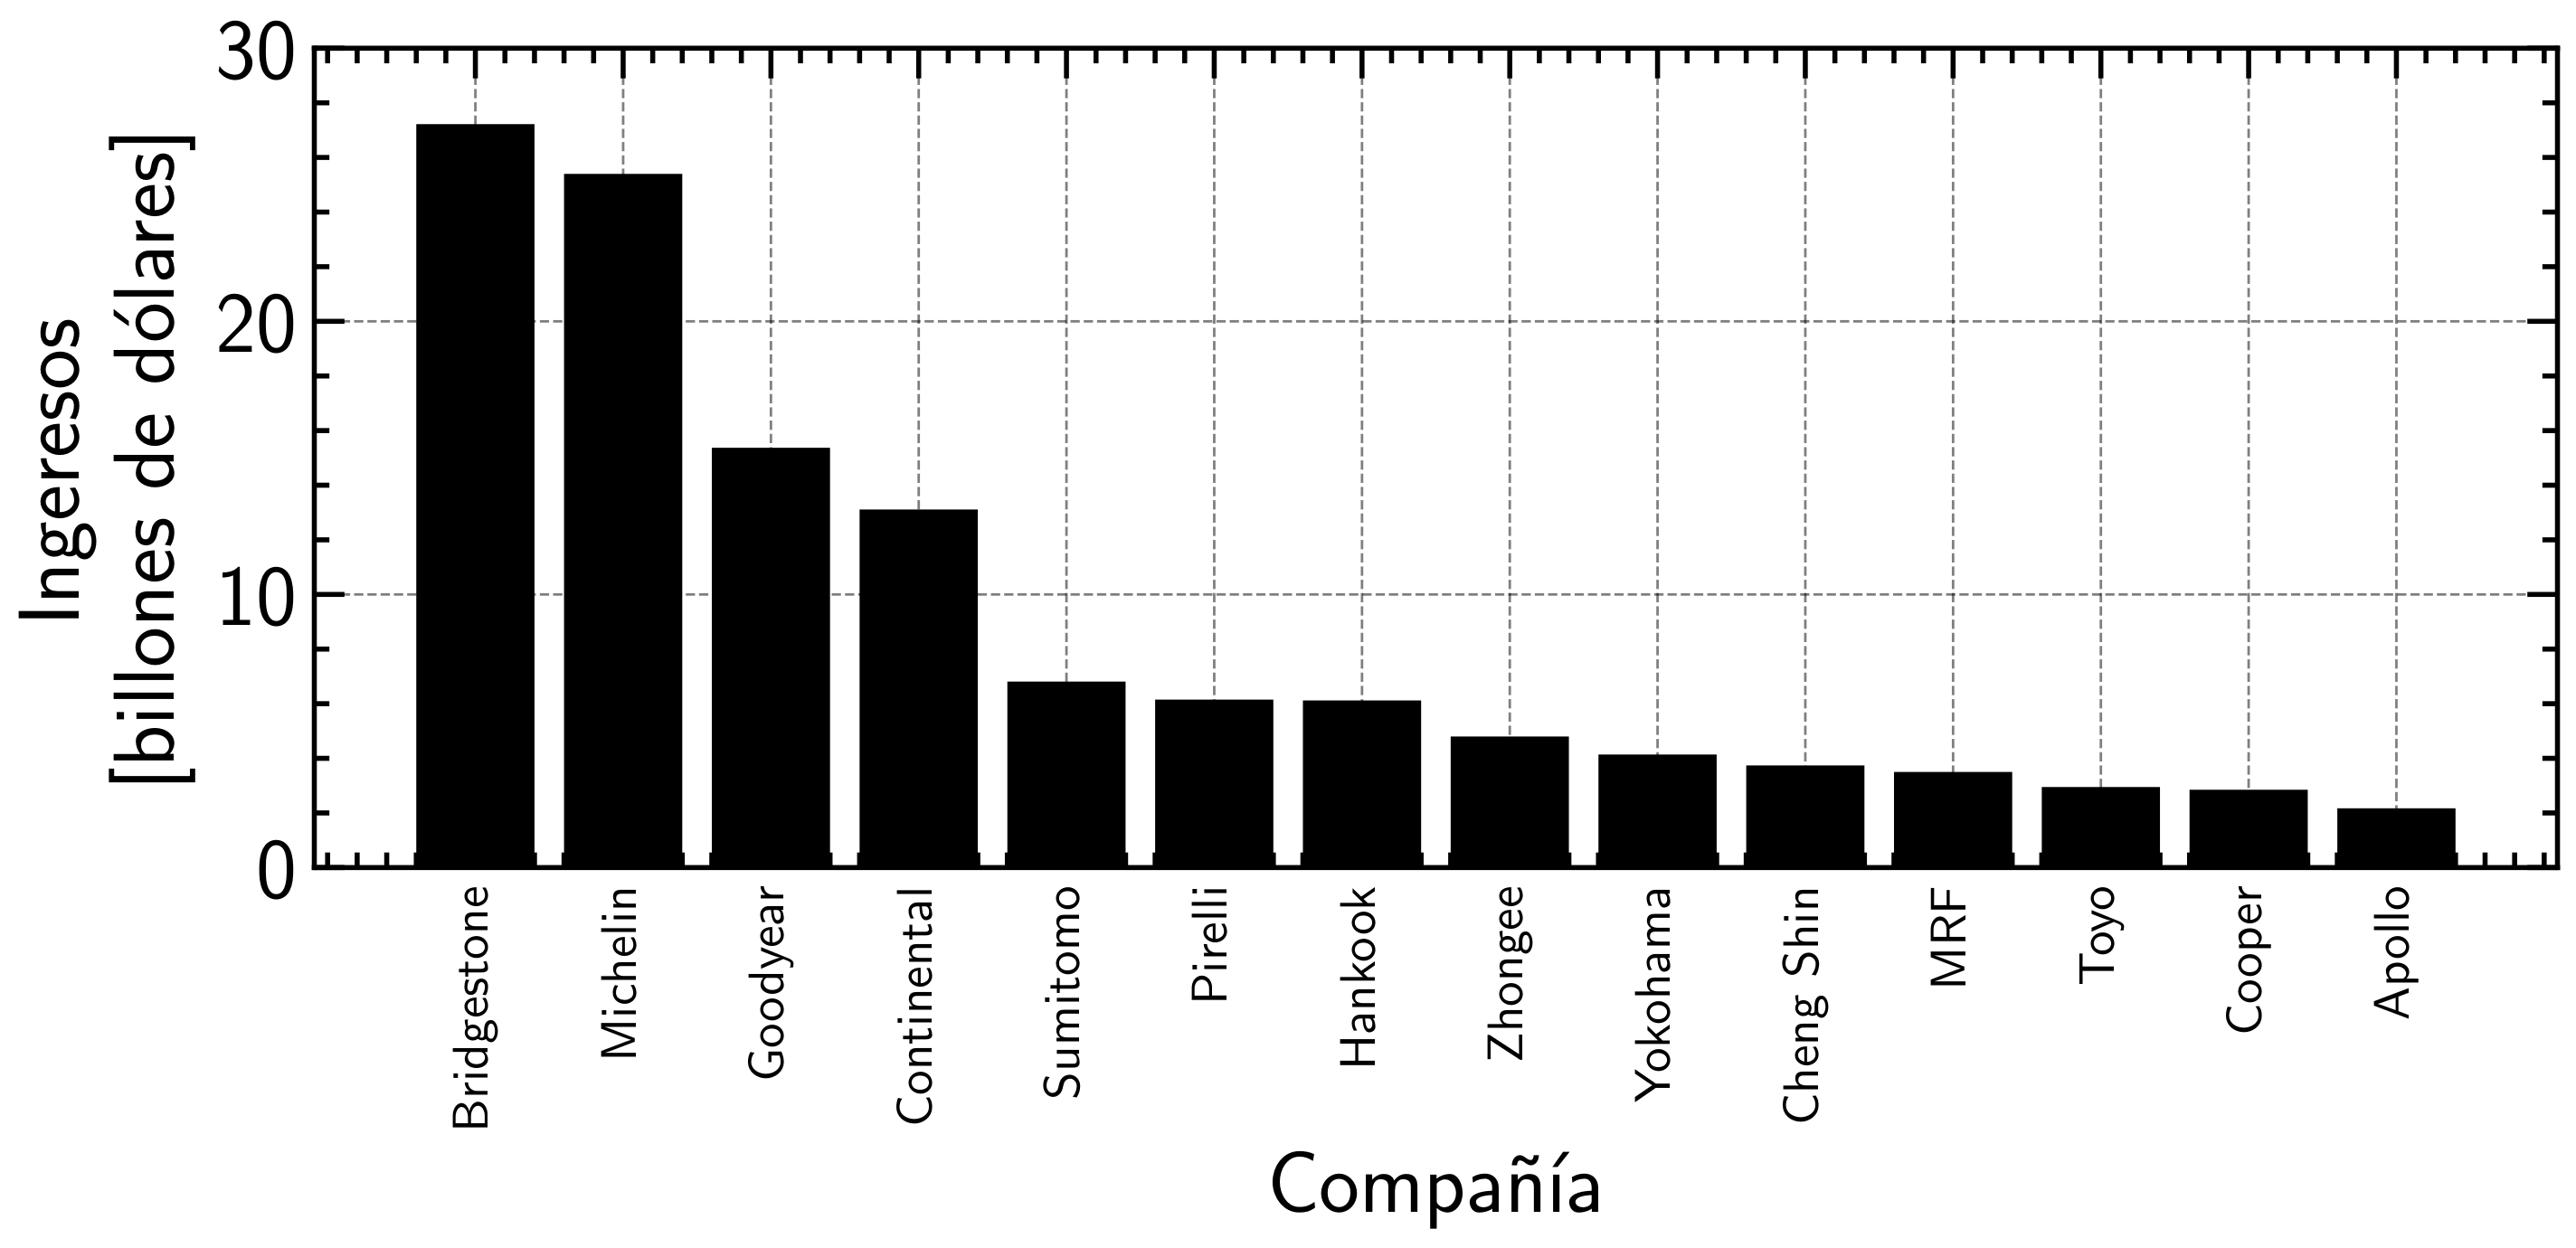
\includegraphics[width=\textwidth]{fig/1_brand.revenue.PNG}
	\end{center}
	\caption{Ingresos de los fabricantes de neumáticos más relevantes en 2019 \citep{rodgers2020tire}.}
	\label{fig:1_brand_revenue}
\end{figure}

La elevada competitividad característica del mercado,
sumada a la emergente comercialización de producto asiático,
incentiva a las establecidas multinacionales, a tomar un enfoque innovativo,
con la intención de mantener su liderazgo \citep{chicu2020current}.
El esfuerzo invertido en innovación,
por una parte, intenta alcanzar sus objetivos
mediante el rediseño y la mejora del producto.
Mientras que por la otra,
trata de optimizar sus procesos y reducir desperdicios,
mediante la automatización y el uso inteligente de los recursos disponibles.

A la hora de implementar mejoras, ya sea a un producto o a un proceso,
la monitorización de los resultados se vuelve esencial.
El producto o proceso experimental debe satisfacer las expectativas del cliente,
y a su vez, cumplimentar la legislación vigente,
como los estándares de calidad y medio ambiente.
La monitorización de estas mejoras implica un coste elevado,
a nivel temporal y económico, ya que estas deben ser puestas a prueba.
En el caso del producto, su industrialización,
supone reservar recursos que podrían ser destinados a la producción regular.
Desde la materia prima utilizada
en la elaboración de estos productos experimentales,
a través de cada máquina ocupada para transformarlo,
hasta llegar al laboratorio de calidad,
donde se realizan ensayos para otorgar feedback a la empresa.

En las empresas de neumáticos, el laboratorio de Calidad del Producto (LCP),
es el encargado de llevar a cabo los ensayos relevantes
para asegurar la conformidad de la producción.
A diario se cerciora de que los neumáticos manufacturados dentro de la planta
cumpla con los estándares de calidad definidos por la compañía.
El laboratorio logra asegurar la calidad del producto,
mediante un control estadístico de las muestras
elegidas al azar por cada gamma de producto.
Paralelamente, una fracción de los recursos disponibles,
es demandada por los proyectos de industrialización.
Obligando al departamento a equilibrar ambas necesidades.

En un entorno con recursos limitados,
donde la demanda no cesa de incrementar,
es cuestión de tiempo que los recursos se agoten
y la capacidad del laboratorio se vea sobrepasada.
Para hacer frente a esta situación,
y poder mantener el esencial ritmo
marcado por los estándares de control de calidad e industrialización,
debe realizarse un escalado de los recursos del LCP.
A fin de que la expansión, de este sistema complejo,
se desarrolle de la manera óptima,
dirigir  un estudio del impacto sobre
las posibles inversiones resulta conveniente.
Debido a que experimentar con el sistema real,
y desarrollar una solución analítica no es factible,
se ha propuesto el uso de la simulación.
Dentro de los tipos de simulación, existen varias alternativas.

\begin{itemize}
	\item Simulación Monte Carlo: Este tipo de simulaciones toma el nombre
		del famoso casino ubicado en Mónaco.
		Este tipo de simulación se caracteriza por desencadenar eventos al azar
		con el fin de obtener los resultados esperados.
		Se emplea con el fin de aproximar
		expresiones matemáticas complejas.
		\citet{owen2016monte} describen la simulación de Monte Carlo,
		como un método para aproximar integrales
		mediante muestras promedio de valores enteros.
		Este método se puede usar, por ejemplo,
		para determinar la probabilidad de que
		un dado obtenga como resultado
		al menos un 5 en 4 de cada diez tiradas.
		El método Monte Carlo es apropiado para sistemas estáticos
		\citep{lawson2008monte},
		es decir, sistemas que no tienen en cuenta el paso del tiempo. 
		
	\item Sistemas Dinámicos (SD): La metodología de los SD trata de capturar
		el comportamiento de un sistema mediante
		su representación en un diagrama de flujo
		\citep{sweetser1999comparison}.
		Esta metodología, toma un enfoque cualitativo,
		apto para gerentes de empresa y organizaciones gubernamentales.
		Los SD están adaptados para sistemas continuos,
		siendo poco prácticos en un ambiente manufacturero,
		donde interrupciones como cambios de turno,
		Reparaciones de máquina, descansos de operario \ldots suceden a menudo.

	\item Simulación de Eventos Discretos (DES):
		Las DES toman el enfoque de representar sistemas reales
		mediante la ejecución y concatenación
		de procesos en un entorno virtual.
		Esta representación computacional se asemeja al sistema real.
		La DES ha demostrado su capacidad de resolver
		problemas de optimización en sistemas estocásticos.
		Como menciona el \citet	{allen2011introduction},
		su versatilidad ha sido demostrada en numerosos ámbitos,
		como aplicaciones militares,
		sistemas sanitarios,
		problemas logísticos
		y optimización de procesos de manufacturación.
\end{itemize}

\subsection{EL LABORATORIO DE CALIDAD DEL \newline PRODUCTO}

A lo largo del proceso de fabricación de una cubierta,
son varios los estándares de calidad que debe cumplir el producto
para que pueda ser vendido en los distintos mercados a nivel global.
Desde la composición química de las materias primas usadas,
hasta las propiedades físicas del producto finalizado,
la certificación de que el producto se halla dentro de
los límites especificados, asegura un producto de calidad.

En el proceso final de control de calidad
que se lleva a cabo en un laboratorio de evaluación del producto,
estos son los ensayos principales.

\begin{itemize}
	\item Ensayos \textit{Endurance}
	\item Ensayos \textit{Rolling Resistance}
	\item Ensayos dimensionales
\end{itemize}

En un LCP,
se debe satisfacer la demanda de ensayos de los siguientes procesos:

Por una parte, los procesos de Conformidad de la Producción (CP),
encargados de aseguramiento de la calidad
del producto destinado a la venta a clientes
Por otra parte, los procesos para el desarrollo de nuevos productos,
propios de las actividades de industrialización (IND),
encargados de desarrollar nuevas líneas del producto,
y optimizar los procesos de producción
mediante cambios controlados que suceden en grupos reducidos.
Finalmente, existen encargos que
no encajan con las 2 anteriores categorías, (EXT).
Para este caso, en el LCP, se ha estimado que,
estas 3 fuentes de muestras de ensayo
suman la cantidad descrita en la Tabla~\ref{tab:2_tbl_actual_demand}.
La cual está cerca, de los límites de capacidad teóricos
para un laboratorio con el equipamiento descrito en
las Tablas~\ref{tab:3_tbl_sim_det} y~\ref{tab:3_tbl_rsrc}.
Las perspectivas de futuro, prevén un incremento continuado de la actividad,
por lo que es habitual que el LCP afronte demandas superiores a su capacidad.

\begin{table}
	\centering
	\caption{Suma de la demanda típica de ensayos en un LCP.}
	\documentclass[varwidth=\maxdimen]{standalone}
\usepackage[utf8]{inputenc}
\usepackage[spanish]{babel}
\usepackage{booktabs}

\begin{document}

\begin{tabular}{ l c }
	\toprule
	Ensayo & Demanda (unds.) \\
	\midrule
	Endurance	& 280 \\
	Rolling		& 760 \\
	Dimensional	& 140 \\
	\bottomrule
\end{tabular}

\end{document}

	\label{tab:2_tbl_actual_demand}
\end{table}

El flujo de los procesos llevados a cabo en el laboratorio,
se representa en la Figura~\ref{fig:2_fc_lep_diagram}.

\begin{figure}
	\begin{center}
		\includestandalone{fig/2_fc_lep_diagram}
	\end{center}
	\caption{Diagrama de flujo de los procesos llevados a cabo en el LCP.}
	\label{fig:2_fc_lep_diagram}
\end{figure}

\subsubsection{Ensayos \textit{Endurance}}
El ensayo \textit{Endurance} esta destinado a medir la fatiga
que pueden llegar a soportar los materiales internos de la cubierta.
Los materiales internos de una cubierta son señalados
en la Figura~\ref{fig:2_tirecs}, como \textit{Steel Belt},
los cuales son capas de hilos de acero entrecruzados que
aportan resistencia a la zona más expuesta de la cubierta.
Las altas temperaturas y cargas a las que son sometidas las cubiertas
producen una separación entre las capas de acero internas.
Esta separación crea una deformación en la superficie de la cubierta.
Cuando una deformación se detecta el ensayo concluye.
Una vez finalizado, un operario corta y pule 2 secciones,
una de ellas se toma en el origen de la separación de las capas interiores,
la restante se toma a 180º del origen de la deformación.

\begin{figure}[H]
	\begin{center}
		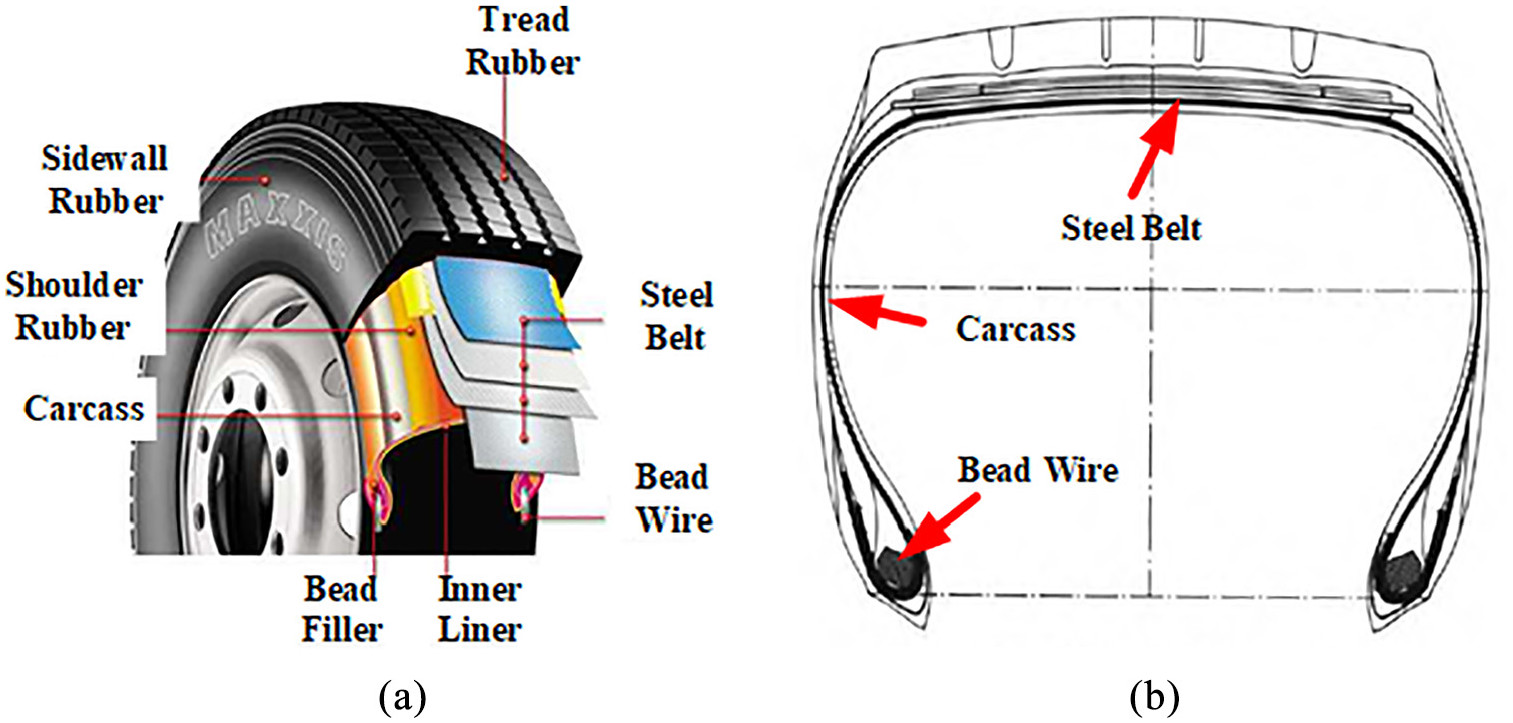
\includegraphics[width=\textwidth]{fig/2_tirecs}
	\end{center}
	\caption{Diagrama de la composición de una cubierta}
	\label{fig:2_tirecs}
\end{figure}

Los ensayos son llevados a cabo en la máquina expuesta
en la Figura~\ref{fig:2_endurance_machine}.
La máquina se encuentra en una sala aislada acondicionada a 40 º$C$.
La carga a la que son sometidas las cubiertas varía durante el ensayo
en incrementos comúnmente llamados pasos.
En la Tabla~\ref{tab:1_tbl_qced_steps} se exponen detalles de cada paso.
La carga a la que es sometida cada cubierta viene determinada
por el índice de carga (LI) grabado en el costado de la cubierta,
a su vez, la velocidad viene determinada por el fabricante.
El LI se muestra en el Anexo~\ref{apnd4}.

\begin{table}
	\centering
	\caption{Pasos de un ensayo \textit{Endurance}.}
	\documentclass[varwidth=\maxdimen]{standalone}
\usepackage[utf8]{inputenc}
\usepackage[spanish]{babel}
\usepackage{booktabs}

\begin{document}

\begin{tabular}{ l c c }
	\toprule
	Paso	& Carga (\%)	& Duración (h) \\
	\midrule
	1		& 66	& 7 \\
	2		& 82	& 16 \\
	3		& 100	& 24\\
	4-12	& +10	& 6 \\
	\bottomrule
\end{tabular}

\end{document}

	\label{tab:1_tbl_qced_steps}
\end{table}

\begin{figure}[H]
	\begin{center}
		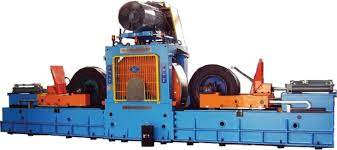
\includegraphics[width=\textwidth]{fig/2_endurance_machine}
	\end{center}
	\caption{Máquina utilizada en los ensayos \textit{Endurance}. 
	Fabricante: RPM. Modelo: TJR2TBY. Especificaciones Técnicas: Anexo~\ref{apnd5}}
	\label{fig:2_endurance_machine}
\end{figure}

\subsubsection{Ensayos Rolling Resistance}
El objetivo de este ensayo es determinar el consumo energético de la cubierta.
El consumo energético está directamente correlacionado
a la fuerza de fricción registrada durante el ensayo.
Según \citet{ydrefors2021rolling}, las variables mas significativas en el valor de \textit{Rolling Resistance} son la presión de inflado y la temperatura de la cubierta.

Para medir el valor de \textit{Rolling Resistance}
se usa la máquina que aparece en la Figura~\ref{fig:2_rr_machine}.
Debido a la sensibilidad del ensayo
a la presión del neumático y la temperatura,
La sala donde se encuentra la maquina tiene que estar acondicionada a 25 º$C$,
y la presión de la cubierta debe ser ajustada con una tolerancia de 0.01 bar.
Para asegurar estas condiciones, las cubiertas deben permanecer
al menos 6 horas dentro de la sala acondicionada antes del comienzo del ensayo.
La presión del neumático se ajusta al
valor marcado en su costado justo antes de comenzar el ensayo.
Finalmente, una vez comenzado el ensayo, se deja transcurrir
el tiempo suficiente para que la cubierta alcance el estado estable.
Una vez alcanzado el estado estable, la máquina toma las mediciones
sobre la fricción y la deflexión de la cubierta.
Al igual que en el ensayo \textit{Endurance}, la carga viene determinada por el LI, y la velocidad por el fabricante.

\begin{figure}[H]
	\begin{center}
		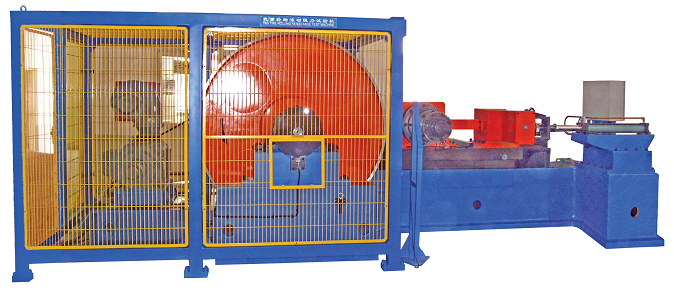
\includegraphics[width=\textwidth]{fig/2_rr_machine}
	\end{center}
	\caption{Máquina utilizada en los ensayos \textit{Rolling Resistance}. Fabricante:RPM. Modelo: TJRRRTBY. Especificaciones Técnicas: Anexo~\ref{apnd5}.}
	\label{fig:2_rr_machine}
\end{figure}

\subsubsection{Análisis dimensional}
El objetivo de este ensayo es verificar que
tanto las dimensiones generales de la cubierta,
como sus componentes internos
quedan dentro de la tolerancia de las especificaciones.

El ensayo se divide en 2 fases.
En la primera fase, El desarrollo de la cubierta es medido a la presión de
inflado especificada en el costado de la cubierta, y a un bar.
Mientras la cubierta conserva su presión de inflado especificada,
se toman los estampados de la huella del neumático introduciendo un folio A3 entre la superficie tintada del neumático, y la prensa.
En la segunda fase, se cortan y se pulen 3 secciones de la cubierta,
para posteriormente ser digitalizadas en un escáner de alta resolución.
Las mediciones a las imágenes obtenidas se realizan mediante un programa.

\subsection{OBJETIVOS}\label{sec_obj}
El objetivo de este trabajo es optimizar los recursos del
típico laboratorio de evaluación de neumáticos,
en el caso de un hipotético crecimiento de la demanda de ensayos.
Esto se consigue mediante el desarrollo de un método basado en una DES.

Para lograr el objetivo final se deberán completar los siguientes subobjetivos:

\begin{itemize}
	\item Modelar los procesos del LCP
		de acuerdo a los fundamentos de una DES,
		obteniendo un modelo ajustado a la realidad.
	\item Definir las variables independientes del proceso,
		que posteriormente serán usadas en la simulación.
	\item Estimar el tiempo de ciclo de cada proceso,
		a través de la asignación de
		distribuciones ajustadas a cada subproceso.
	\item Definir las variables dependientes
		que otorgara el sistema a la salida.
	\item Desarrollar un programa de simulación en el entorno de Python
		mediante el uso de la librería Simpy.
		Dicha simulación, será capaz de emular
		los distintos escenarios propuestos durante el desarrollo.
	\item Proponer una alternativa de la distribución de
		los recursos descritos al comienzo del trabajo, 
		para asegurar la capacidad del LCP cuando en el caso de que aumente la
		demanda de ensayos.
\end{itemize}
